\chapter{Implementation Details}

\section{Architecture}

\begin{wrapfigure}{r}{0.48\textwidth}
    \vspace{-12pt}
    \centering
    
\includegraphics[width=0.48\textwidth]{img/fig_5.1.png}
    \caption{
        Denoised results for both skip connection variants.
        Both images are obtained using SG-DIP\@.
        The ECA-based variant retains more structural details compared to the convolution-based approach.
    }\label{fig:ECA}
\end{wrapfigure}
All architectures in our experiments use a fully-convolutional encoder-decoder network with skip connections, following the U-Net~\cite{U-Net} architecture.
The encoder progressively downsamples the input using strided convolutions, increasing the number of feature channels while reducing spatial resolution.
The decoder then upsamples the feature representations back to the target resolution using bilinear upsampling followed by additional convolutions.
Skip connections are employed between corresponding encoder and decoder layers, bypassing the bottleneck to preserve fine-grained details.
This helps retain spatial information that would otherwise be lost due to downsampling, thereby improving reconstruction quality.
We find that parameterizing these skip connections is crucial for achieving strong denoising performance.
While the original DIP paper employs $1 \times 1$ convolutions in the skip connections, we also explore a variant that replaces these convolutions with ECA blocks.
We find that both variants yield comparable performance in terms of PSNR and SSIM\@; however, ECA blocks often contribute to better preservation of fine details, as shown in Figure~\ref{fig:ECA}.

As in the original DIP paper, Batch Normalization is applied throughout the network and all activation functions are LeakyReLU~\cite{LeakyReLU}.
LeakyReLU extends ReLU by allowing a small slope for negative values, ensuring non-zero gradients throughout the domain.
Formally, it is defined as
\begin{equation}
    \varphi(x) = \begin{cases}
        x &\text{if}\ x \geq 0\\
        \alpha x &\text{if}\ x < 0,
    \end{cases}
\end{equation}
where $\alpha = 0.2$ in our case.
Unless noted otherwise, all experiments employ the architecture visualized in Figure~\ref{fig:architecture}, implemented using PyTorch~\cite{PyTorch}.
Optimization is performed using the Adam optimizer~\cite{Adam} with a learning rate of 0.01.

\begin{figure}
    \centering
    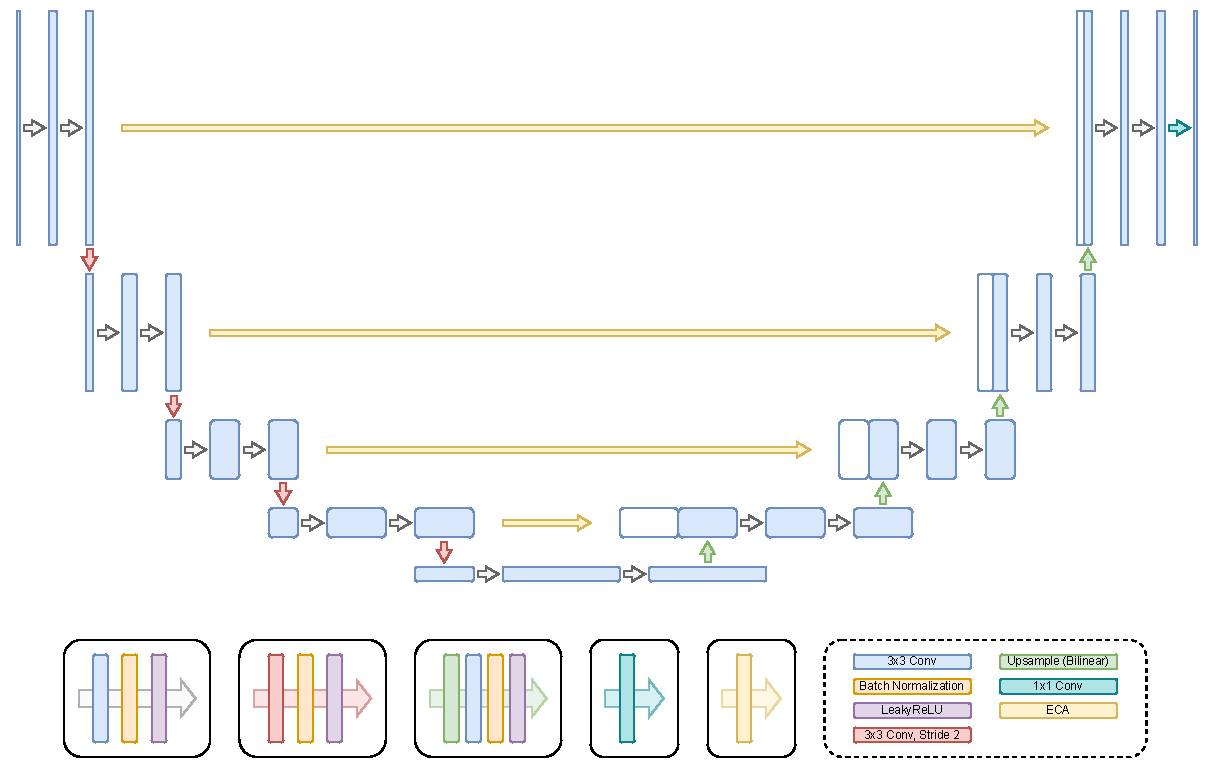
\includegraphics[width=\textwidth]{img/fig_5.2.pdf}
    \caption{
        Architecture used in our experiments.
        Each blue box corresponds to a multi-channel feature map.
        White boxes represent copied feature maps, reweighted using ECA\@.
        Different colored arrows represent different operations, visualized in detail in the boxes below.
        Figure adapted from~\cite{U-Net} and~\cite{DIP}.
    }\label{fig:architecture}
\end{figure}

\section{Metrics}

\section{Datasets}

\section{Preprocessing}
